%%%%%%%%%%%%%%%%%%%%%%%%%%%%%%%%%%%%%%%%%%%%%%%%%%%%%%%%%%%%%%%%%%%%%
%%%%%%%%%%%%%%%%%%%%%%%% COMMUNITY DETECTION %%%%%%%%%%%%%%%%%%%%%%%%
%\section{Community structure in the brain}
\section{Modularity of brain networks}
A systematic analysis of the structure of neural systems in different organisms points out that modularity is a factor that shapes neural networks from the small nematode worm \emph{Caenorhabditis Elegans} to the most complex human brain~\cite{meunier2010,towlson2013,park2013}. 
Topological network analyses suggest indeed that modular and hierarchical structural networks are particularly well-suited for the functional integration of locally specialized neural operations that underlie cognition~\cite{sporns2004,sporns2004a,bullmore2012,meunier2010,bressler2010}.
In this respect, brain function or cognition can be described as global integration of local integrators~\cite{park2013}.

Among the many advantages of a modular organization of the brain, three are of greatest importance and strictly intertwined: adaptability, robustness and wiring cost economy.
Firstly, from an evolutionary perspective, a modular architecture is highly adaptable to an ever changing environment and variable loads of cognitive demands.
From generation to generation, modules that were already well-fit to the environmental conditions were selected and passed, while others were only slightly rewired through the natural selection mechanisms. This pressure, together with the imperative of a reduced wiring cost have crucial to select an architecture that converged to a construction of tightly connected sub-networks loosely connected to each others~\cite{clune2013}.
Computational studies have shown that a modular organization emerges spontaneously in complex brain networks, promoting flexibility to an ever-changing outside environment~\cite{kashtan2005,kashtan2007} and maximizing bidirectional information exchange between neural populations~\cite{yamaguti2015}.

A second benefit of modularity is robustness as it facilitates evolvability and robust traits like the multiscale modular architecture are often selected by evolution~\cite{kitano2004,betzel2016}.
Indeed, keeping a system compartmentalized can limit the influence of external sources of perturbation, thus bounding the interdependence of biological processes going on in each unit~\cite{kirschner1998}, and promoting greater resilience in the context of continuous genetic and developmental changes.
In addition, swapping and rewiring maladaptive modules is less demanding that restructuring the whole system.
A general problem in the acquisition of new skills is the phenomenon of catastrophic forgetting, by which newly acquired skills come at the expense of others~\cite{french1999}.
In the case of neural networks it has been shown that a modular organization helps to avoid catastrophic forgetting of newly learned skills, whereby new skills are learned by slightly rewiring existing modules, rather than changing the overall organization~\cite{ellefsen2015}.
Local disruptive modification may only affect one module, whereas the others are preserved from the insult~\cite{stam2014}.
In case of externally or internally generated fluctuations, a modular architecture prevents functional disruption of the network leading to the possible death of the organism.

Thirdly, the spatial and metabolic constraints of neuronal wiring are factors that deeply shaped the brain architecture~\cite{bullmore2012,stam2012}. Computational and empirical studies converged on the result that a multiscale organization of modules inside modules is the one that satisfies the constraints imposed by minimization of energetic cost and spatial embedding~\cite{pan2007,bullmore2012,doucet2011,betzel2017,kaiser2006}.
Here, wiring cost must not only be intended as the physical volume of axons and synapses but also be considered in terms of energetic demand for signal transmission, additional processing cost for noise correction over long distance signalling and sustenance of the necessary neuroglia that supports neuronal activities~\cite{bullmore2012}. In terms of wiring cost reduction, modular networks emerge naturally when minimizing the average path length and the total number of links, while maximizing robustness against perturbations in node activity.
By way of example, in the field of robotics, spontaneous structural modularity of neural networks controllers emerge from evolutionary optimization when successful robot behaviour is encoded as fitness function~\cite{bongard2011}.

\bigbreak

Application of resting state fMRI has allowed the identification of various modules in human functional connectivity.
These spatially distinct modes that demonstrate synchronous BOLD fluctuations, consist in strongly correlated, anatomically separated, possibly remote regions of the brain~\cite{biswal1995,raichle2001,fox2005,biswal2012}.
Various methods exist for analyzing resting-state data, including seed-based approaches~\cite{biswal1995,raichle2001}, independent component analysis~\cite{beckmann2005,damoiseaux2006} and graph-based methods~\cite{stam2007,bullmore2009}. They have generally shown that the human brain is functionally organized in a number of interconnected regions with boundaries that reflect specific aspects of cognitive and behavioural aspects~\cite{tomasi2012,alnaes2015,crossley2013a}.
The first analysis method ever used was the seed-based approach~\cite{biswal1995}, which has been applied in numerous studies~\cite{raichle2001}.
This technique is based on the correlation of voxels within selected regions of interest (ROIs), with the average BOLD signal from all other voxels in the brain.
An accurate thresholding is then needed to identify voxels that are significantly correlated with the region of interest.

Another widely used approach is the decomposition of the endogenous BOLD fluctuations by means of Independent Components Analysis, a technique that aims at maximizing statistical independence between time courses of single voxels and that can identify separate spatial modes~\cite{damoiseaux2006,beckmann2005,calhoun2013}.
Yet, ICA with its variants still relies on user experience to discern important components from noise~\cite{lee2013} and despite some notable attempts to identify noise~\cite{thomas2002,tohka2008}, like seed-based approaches, does not yield any information on the hierarchy of modes, nor on their relation.
Moreover, largely overlapping results can be obtained by ICA and seed-based approaches~\cite{rosazza2012}.

The evidence of modules in human functional networks is based on their robustness and consistency within a variety of MRI protocols, different analysis methods, and MRI scanners. 
Differently from structural networks, since functional networks do not measure physical relations with associated metabolic or material cost, they may feature long-distance connections~\cite{dehaene1998,varela2001} and ever changing patterns.
The majority of analysis techniques are concordant in identifying a set of robust functionally linked regions, or \emph{modules} in resting state networks.
These modules, roughly highlighted with coloured ellipses in Figure~\ref{fig:vandenheuvelnetworks} span the primary somatosensory network, the primary visual and extra-striate network, a network consisting of bilateral temporal/insular areas and anterior cingulate cortex regions, left and right lateralized networks consisting of superior parietal and superior frontal regions (often reported as one single network) and the so-called default-mode network spanning precuneus, medial frontal, inferior parietal cortical regions and medial temporal lobe.
\begin{figure}[!htb]
\centering
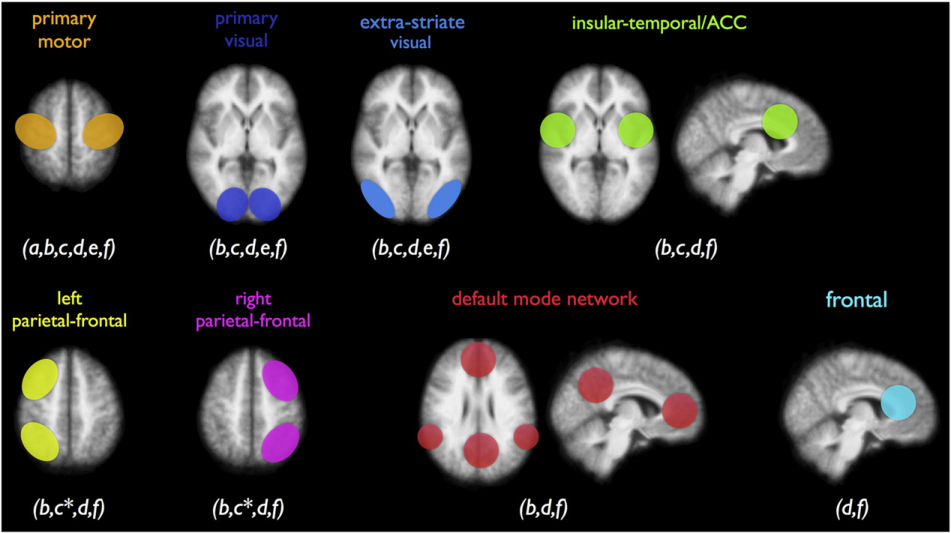
\includegraphics[width=1.0\textwidth]{images/vandenheuvel_networks.pdf}
\caption{Functional modules of the resting state brain, averaged over different studies and protocols, and visualized roughly on a brain template to indicate their anatomical position. Figure taken from~\cite{vandenheuvel2010}.}
\label{fig:vandenheuvelnetworks}
\end{figure}
The Default Mode Network, or DMN, firstly identified by Raichle~\cite{raichle2001} with positron emission tomography and then confirmed by Greicius et al. using fMRI~\cite{greicius2003} is one of the most consistent networks among a variety of studies. It comprises a group of spatially remote brain regions that show higher levels of correlation when the brain is not involved in any particular cognitive or behavioural task.
For this reason, it is hypothesized that there are two opposing concurrent large scale modes, one including the DMN, indicated as ``task-negative'' or ``intrinsic'' system, and the other comprising regions involved in attentional and task evoked activities, dubbed ``task-positive'' or ``extrinsic'' system~\cite{power2011,fox2002,golland2008}.
The Default Mode Network or DMN (Figure~\ref{fig:vandenheuvelnetworks}) is thought to be connected to high-level cognitive functions, given its specific traits of structural links to associative brain regions and that the DMN may support internal mental processing like mind-wandering, abstract thinking and planning of events in the future~\cite{gusnard2001,buckner2008}.
Additionally, evidence has pointed to disruptions in the DMN with people with Alzheimer's disease~\cite{buckner2008}, autism spectrum disorders~\cite{washington2014} and schizophrenia~\cite{garrity2007}.

Apart from the DMN and networks for the primary sensory areas, other networks have different roles, many of which are partly speculative.
Subcortical communities have also been identified with rs-fMRI: an appropriate ICA seeding, makes possible to observe functional modules located at the thalamus and hippocampus~\cite{lee2012}.
Modules in functional brain networks have been explained as the possible basis of a large variety of neural processes.
By way of example, certain functional processes, like colour vision, have been described as anatomically localized~\cite{zeki1998}, while others, like working memory, have been proposed to involve more globally integrated processing systems~\cite{dehaene1998,baddeley2003}.
Interestingly modules of functional brain networks are non-static as recent studies found that they tend to become less and less modular with ageing~\cite{meunier2009a,song2014}.
In all respects, the experimental indication of the modular organization is a powerful and robust marker against which to measure the health of the brain. 
Thus, modularity is not only a biologically plausible feature but it is very likely necessary to maintain the rich repertoire of cognitive tasks that our brain engages in every day of our life.

Modeling of resting state networks by means of graph-theory provides a compelling alternative to seed-based and ICA approaches.
Within this framework ROI are nodes of a network, connected by edges of weight proportional to the strength of correlation between ROIs.
Graph-theory offers a wide amount of measures to characterize functional connectivity networks and in particular a wealth of methods to identify communities, subsets of nodes which are more strongly correlated between each other, than with external nodes~\cite{bullmore2009,stam2014,sporns2016}.

Interestingly, the size distribution of the functional modules has never been analyzed in details, especially when graph-theoretical methods were applied.
This is the case of one of the most fortunate and widely adopted method to identify modules in functional networks, Newman's Modularity~\cite{newman2006}.
Despite its popularity and merits, Newman's approach presents some important limitations.
Already at an early stage, Modularity-based methods were shown to suffer from a resolution limit, as they fail to identify modules that are smaller than a scale that depends on the size of the overall network~\cite{fortunato2007}.
As a consequence, even unambiguously defined modules, like complete sub-graphs or cliques, may be unduly merged into larger communities when they are too small compared to the size of the network.
Subsequent work by various groups has shown that the resolution limit is quite pervasive~\cite{lancichinetti2009,traag2011,squartini2015,lancichinetti2011,kawamoto2015}, and affects, to a different extent, many other methods, including Reichardt and Bornholdt’s~\cite{reichardt2006}, Arenas and Gomez'~\cite{arenas2008}, Ronhovde and Nussinov's~\cite{ronhovde2009}, Rosvall and Bergstrom's (\emph{Infomap})~\cite{rosvall2008,kawamoto2015} and others.

Fixes have been proposed to circumvent the resolution limit, including the introduction of a tunable parameter that enables analysis of the network at an adjustable resolution level~\cite{reichardt2006,ronhovde2010,yeo2011}. However, this requires prior knowledge of the expected size of the communities for the tuning of the resolution parameter. Moreover, it has been shown that an  adjustable resolution parameter may reduce the tendency to merge small clusters, but only at the cost of unduly splitting large clusters~\cite{lancichinetti2011}. Adjustment of the resolution parameter is an attempt to balance these two biases, but multiresolution methods fail to recover community structures comprising heterogeneous distributions of cluster sizes~\cite{lancichinetti2011}. 
However, real-world networks are characterized by the coexistence of clusters of very different sizes, and no single parameter can adapt to the variety of network topologies observed in nature.
Hence, the resolution limit may represent a critical shortcoming for the study of brain networks and is likely to have affected many of the studies reported in the literature.

In the following sections I'm going to illustrate the current graph-theoretical approaches for community detection in networks and to discuss the theory of community detection, highlighting the practical problems of Modularity maximization.



		% A number of other resting-state networks has been identified

		%  Studies have hypothesized that there are
		% 2 large opposing systems in the brain, one including the DMN and
		% the other composed of attentional or task-based systems, such as
		% somatosensory, visual, or attention RSNs. Terms used to refer to
		% these systems include “task-positive” and “task-negative”4,12,13
		% and “intrinsic” and “extrinsic.”14,15
		% Several other RSNs have been identified. The somatosensory
		% network, studied first by Biswal et al,1 includes primary and
		% higher order motor and sensory areas (Fig 1B). The visual network
		% is highly consistent across various studies and spans much of
		% the occipital cortex (Fig 1C).2-6An auditory network consisting of


		% Another popular approach is ICA,2,10 a mathematical technique
		% that maximizes statistical independence among its components.
		% For RS-fMRI data, ICA can be used to spatially identify distinct
		% RSNs. Compared with seed-based methods, ICA has the advantage
		% of requiring few a priori assumptions but does compel the
		% user to manually select the important components and distinguish
		% noise from physiologic signals. Some studies have aimed to
		% automate this process and use ICA as a method for identifying
		% noise within the BOLD signal.33-36 Despite the differences in the 2
		% approaches, Rosazza et al37 showed that the results of seed-based
		% analysis and ICA are significantly similar in a group of healthy
		% subjects.
		% Graph methods provide a distinct alternative to seed-based
		% analyses and ICA.4,38-44 This approach views RSNs as a collection
		% of nodes connected by edges. With RS-fMRI data, ROIs can be
		% represented as nodes, and correlation between the ROIs, as the
		% connectivity of the edges. Connectional characteristics of the
		% graph can then be computed.44 Examples of measures of interest
		% include the average path length, a measure of global connectedness,
		% which is the average length of the shortest connection between
		% all pairs of nodes.44 Another measure of interest is the clustering
		% coefficient, which is related to the connectedness of
		% neighboring nodes and reflects the presence of smaller subgraphs.44
		% Using these techniques, several studies have demonstrated
		% that the brain exhibits a small world topology. Small world
		% topology, which was first described in social networks, allows each
		% node to have a relatively low number of connections while still
		% being connected to all other nodes with a short distance. This is
		% achieved through the existence of hubs, which are critical nodes
		% with large numbers of connections, that allow high levels of local
		% connectivity.39,45 Small world networks have high clustering coefficients
		% implying high levels of local connections (ie, cliques or
		% groups) and an overall short distance between any 2 nodes, or a
		% small average path length.40-42


%%%%%%%%%

% % Unfortunately, until recently most of the studies in animal models were based on anatomical connectivity measured by means of post-mortem inspections.
% % While in the past, histological staining was the most adopted methodology to inspect the wiring of white matter in the animal brain, the last few decades have seen the rising of fluorescence based tract-tracing, that evolved to a level where single axons can be traced with unprecedented precision~\cite{oh2014}.
% % Not only methods to investigate the structural connectivity have greatly evolved, but also new cellular resolution recording systems, like light-sheet microscopy~\cite{ahrens2013}, real time in-vivo two-photon cortical imaging~\cite{dombeck2010,leinweber2014} and spike time series recordings on multielectrode arrays~\cite{shimono2015}.
% % All these techniques take part in the quest to shed light on the relation between functional networks and their underlying anatomical substrate.

% After the discovery of low frequency fluctuations of the BOLD signal of the brain at rest~\cite{biswal1995}, 
% In humans, non-invasive studies of the brain community structure largely reflect the analytical methodologies adopted in animals.
% In both contexts, functional connectivity is suggested to describe the relationship between neuronal activity patterns of anatomically separated regions that reflect the level of information exchange between them.
% The decomposition of the endogenous fluctuations of the BOLD signal at rest by means of independent components analysis (ICA), showed a repertoire of \emph{spatial modes}, clusters of brain regions whose neural activity oscillates synchronously. These patterns of spontaneous coupled oscillations are strongly correlated between anatomically separated, possibly remote regions of the brain~\cite{biswal1995,raichle2001,fox2005,biswal2012}. Additionally, these patterns of functional connections that derive from a modular architecture of the brain, are themselves modular. A submodule (or subnetwork), often called community in graph theory, comprises synchronously active voxels. The enduring and stable synchrony within those voxels is thought to reflect local integration processes



% The evidence of modules in functional brain networks has been explained as the possible basis of a large variety of processes. By way of example, certain functional processes, like color vision, have been described as anatomically localized~\cite{zeki1998}, while others, like working memory, have been proposed to involve more globally integrated processing systems~\cite{dehaene1998,baddeley2003}.
% Interestingly modules of functional brain networks are non-static as recent studies found that they tend to become less and less modular with aging~\cite{meunier2009a,song2014}. 
% In all respects, the experimental evidence of the modular organization is a powerful and robust marker against which to measure the health of the brain. 
% Thus, modularity is not only a biologically plausible feature but it is probably necessary to maintain the rich repertoire of cognitive tasks that our brain engages in every day of our life.

% Despite the biological evidence of modularity in brain networks, the number of modules returned by clustering methods is often chosen in advance, based on the experience of the researcher, even if some complex approaches are available~\cite{still2004}. 

%%%%%%%%%%%%%%%%%%%%%%%%%%%%%%%%%%%%%%%%%%%%%%%%%%%%%%%
%%%%%%%%%%%%%%%%%%%%%%%%%%%%%%%%%%%%%%%%%%%%%%%%%%%%%%%
%%%%%%%%%%%%%%%%%%%%%%%%%%%%%%%%%%%%%%%%%%%%%%%%%%%%%%%

\section{Community detection in networks}
\label{sec:communitydetectioninnetworks}
The process of grouping nodes in a graph to establish their common behavioral properties is a popular technique that goes under the name of \emph{community detection}.
Following the initial work by Hilgetag~\cite{hilgetag2000a} dubbed OSA (Optimal Set Analysis), several graph theoretical methods have been deployed to investigate the modular structure of structural and functional brain networks~\cite{meunier2009,meunier2010,power2011,stam2007,stam2014}.
Typically, these methods rely on the optimization of a fitness function that measures the quality of a network partition against that of an ensemble of randomized networks with similar statistical properties, called the ``null model''.
Optimization of the fitness function of choice is often computationally demanding and scales steeply with increasing network size.
Hence, heuristics are needed to calculate nearly optimal partitions of large networks, like those derived from neuroimaging data, within reasonable computation time~\cite{blondel2008,rosvall2008,raghavan2007}.
As the definition of community is not unambiguously stated, it is therefore, important to have a quantitative way to evaluate the goodness of such clusterings.

A global criterion for the definition of communities in networks can be thought in terms of a fitness function defined over the clustering.
A \emph{quality function} is a function $\mathcal{Q}$ that given a clustering of a graph $\zeta$ returns a scalar number. Usually one identifies ``good'' clusterings with high scores of the quality function and ``bad'' clusterings with low scores. In this sense, it is possible to rank partitions from bad to good, although is important to stress that the definition of good or bad clusterings is an \emph{ill-posed problem} as every quality function puts emphasis on some features and perhaps not on others. 
Here and in the following sections, it must be stressed that the concept of quality function and community detection methods are separate as the first is a way to assess the goodness of a partition while the second relies on the definition of a quality function to design efficient algorithms and heuristics to find such good partitions.

One of the most important properties of a quality function is when it can be expressed as a sum over communities.
Such quality functions are dubbed \emph{additive}: for a generic function of a cluster, or subgraph, $f(\zeta_i)$, an additive quality function specify the goodness of a clustering as the sum of $f$ over the distinct communities as follows:
\begin{equation}\label{eq:additive_quality}
\mathcal{Q} = \sum \limits_{\zeta_c \in \zeta} f(\zeta_c).
\end{equation}
The majority of quality functions are additive, even if this requirement is not fundamental.
In the next section, we explore the properties of some of the most important additive quality functions that emerged from the literature of this decade.

\subsection{Spin glass based quality functions}
The simplest requirement of a quality function is to put emphasis on intracluster edges and penalize intercluster edges.
In this terms, local optima of the quality function should correspond to partitions where the communities emerge as dense areas in the network loosely connected among them. A framework grounded in statistical mechanics for the definition of suitable quality functions for community detection that meet these requirements has been introduced by Reichardt and Bornholdt (RB)~\cite{reichardt2006}.

In the RB model the problem of community detection is cast in terms of finding the \emph{ground state} of a spin glass, a model describing the behavior of large sets of interacting microscopic magnets.
Actually, the properties of spin glass models are subject of extremely intensive research in the last decades as their applications range from matter and nuclear physics to neural networks. Here we present only their salient application to community detection and refer the reader to cover the details of the model in other more specialized resources~\cite{mezard1990}.

A spin glass model is based on the definition of an Hamiltonian, a multi-variable scalar function that describes the total energy of the physical system with the configuration of its internal components.
In our case, the internal components of the system are the nodes. The configuration of the system is then expressed by the community affiliation vector $\boldsymbol\sigma$, meaning that node $i$ stays in the community $\sigma_i$.
The Hamiltonian used by Reichardt and Bornholdt (RB) counts four different contributions. The first two contributions act at intracluster level, positively weighing intracluster edges and negatively weighing intracluster non-edges with coefficients $a_{ij}$ and $b_{ij}$ respectively. The third and fourth contributions work on intercluster edges and non-edges, weighing them with factors $c_{ij}$ and $d_{ij}$. The general form of the RB model is then expressed by the following Hamiltonian:
\begin{align}\label{eq:hamiltonianspinglass}
\mathcal{H}^{\textrm{RB}}(\boldsymbol \sigma) = - \sum_{(i,j)\in V^2} & \left[ a_{ij} A_{ij} - b_{ij}(1-A_{ij}) \right] \delta(\sigma_i,\sigma_j) + \nonumber \\ &  \left[ (c_{ij} A_{ij} - d_{ij}(1-A_{ij}) \right] (1-\delta(\sigma_i,\sigma_j)),
\end{align}
with the convention that lowest energy states correspond to best community assignments.
Rearranging Eq.\ref{eq:hamiltonianspinglass} and discarding the terms independent of the partition into a constant $H_0$, one then gets a simpler expression for $\mathcal{H}^{\textrm{RB}}(\sigma)$:
\begin{equation}\label{eq:rbspinglass}
\mathcal{H}^{\textrm{RB}}(\boldsymbol \sigma) = -H_0 - \sum \limits_{(i,j)\in V^2} \left[ \alpha_{ij} A_{ij} - \beta_{ij} \right] \delta(\sigma_i,\sigma_j),
\end{equation}
where the two parameters $\alpha_{ij}=a_{ij}+b_{ij}+c_{ij}+d_{ij}$ and $\beta_{ij}=b_{ij}+d_{ij}$ depend on the \emph{null model} one would like to compare with, i.e. the probability that an edge exists between $i$ and $j$ after random edge rewiring. Hence, a null model provides a mean to compare a specific set of features of a graph, with its randomized version that should specifically lack those features.

It's possible to express any quality function in the form of Eq.~\ref{eq:rbspinglass} as an additive quality function by setting $\alpha_{ij}=1$, $H_0=0$ and moving the summation indexes over the communities rather than over the pairs of nodes, as the sum is only over intracluster edges. The resulting Hamiltonian, expressed here as $\mathcal{H}^{\textrm{RB}}_{\textrm{reduced}}(\sigma)$, then reads:
\begin{equation}\label{eq:rbspinglass2}
\mathcal{H}^{\textrm{RB}}_{\textrm{reduced}}(\sigma) = -\sum_{(i,j) \in V^2} \left[ A_{ij} - \beta_{ij} \right] \delta(\sigma_i,\sigma_j) = - \sum \limits_{c}^C \left[ m_c - \left< m_c \right> \right].
\end{equation}
where $m_c=\sum_{ij}A_{ij}\delta(\sigma_i,c)\delta(c,\sigma_j)$ represents the number of links inside community labeled by $c$ and $\left <m_c \right >=\sum_{ij}\beta_{ij}\delta(\sigma_i,c)\delta(c,\sigma_j)$ is the expected number of links in community $c$ as prescribed by the null model $\beta_{ij}$\footnote{Here and for the rest of the work, we set $P_{ij}:=\beta_{ij}$ for agreement with more conventional notation of null models}. 
Among the additive quality functions that show up in the form of~\ref{eq:rbspinglass2}, the most important and popular is the \emph{Newman-Girvan's Modularity}.

\subsection{Newman-Girvan Modularity}\label{sec:newman_modularity}
Newman-Girvan Modularity (or simply Modularity)~\cite{newman2006}, denoted here and for the rest of the work by $Q^N$, is based on the idea that a network obtained by randomly reshuffling the original graph edges while keeping the same degrees sequence, should not display any community structure. 
An important consequence of such randomization is that any stub in this null model, dubbed ``configuration model'' is equally likely to be connected to any other~\cite{newman2010book}. Thus, in absence of correlations, the probability that two nodes are connected is expressed by:
\begin{equation}\label{eq:configuration_model}
P_{ij} = \frac{k_i k_j}{2m},
\end{equation}
where $k_i$ and $k_j$ are the degrees of node $i$ and $j$. The ``configuration model''  is of great importance in network science as it assigns a higher probability of linking to nodes with high degrees, a feature that is compatible with most real world networks~\cite{newman2010book}.
The motivations of the configuration model are addressed in details in section~\ref{sec:configuration_model}.

In terms of a spin glass model, Modularity measures the deviation from the observed intracluster density with respect to the expected intracluster density specified by the configuration model. Modularity is described in the form of~\ref{eq:rbspinglass2} but normalized by the number of edges in the graph, taking the form described in Eq.~\ref{eq:newmanmodularityspinglass}.
\begin{equation}\label{eq:newmanmodularityspinglass}
Q^N =  \frac{1}{2m} \sum_{ (i,j) \in V^2} \left[ A_{ij} - \frac{k_i k_j}{2m} \right] \delta(\sigma_i,\sigma_j),
\end{equation}
whereby optimal partitions have high values of $Q^N$. As already done in Eq.~\ref{eq:rbspinglass2}, Modularity can alternatively be expressed, as sum over communities of the difference of two terms:
\begin{equation}\label{eq:newmanmodularity}
Q^N = \sum_{c}^{|C|} \left[ \frac{m_c}{m} - \left( \frac{K_{\textrm{int}}(\mathcal{G}_c)}{2m} \right)^2 \right].
\end{equation}
Modularity takes values in the range $[-0.5,1]$, then a good partition should have $Q^N$ values close to unity, identifying groups with much more internal connections than expected at random. In contrast, a bad partition with $Q^N$ close to zero should identify groups with no more internal connections than we expect at random.
In the next sections, we will challenge this idea and show that this observation has led to false statements, as a general phenomenon dubbed \emph{resolution limit}, heavily affects any quality function based on comparison with global null models.
Specifically, in the case of Newman's Modularity, the resolution limit hampers its ability to detect modules smaller than a scale determined by the size of the graph.

\subsection{The configuration model}\label{sec:configuration_model}
A central property of the configuration model is the probability $P_{ij}$ of the occurrence of an edge between two specified vertices $i$ and $j$.
In absence of correlations, as prescribed by the random reshuffling imposed by the configuration model, the probability that a stub emerging from vertex $i$ is connected by an edge to any of the stubs of vertex $j$ is $k_j/(2m-1)$ as there are $2m-1$ stubs in total.
Therefore the total probability that vertex $i$ and vertex $j$ are connected by an edge is the product of the stub probability times the number of stubs from vertex $i$, namely 
\begin{equation}\label{eq:configuration_model_probability}
P_{ij} = \frac{k_i k_j}{2m-1} \approx \frac{k_i k_j}{2m}.
\end{equation}
Although the configuration model is most frequently applied to \emph{simple graphs} (Figure~\ref{fig:simple_unweighted_graph}), the configuration model implies that the randomization is carried over the space of \emph{loopy multigraphs} (Figure~\ref{fig:loopy_multigraph}).
The rewiring probability considers indeed that the stubs of nodes can be reconnected both to the same source vertex (self-loops) or added to already existing edges (multi-edges).
Consider for example the set of matchings on six stubs that form a triangle graph as illustrated in Figure~\ref{fig:configuration_model_stubs}. The configuration model chooses each distinct edge stubs labeling with equal probability. However, not only the first eight distinct reshuffled labelings are possible under configuration model (Fig.\ref{fig:reshuffle_simple_graphs}) but many other distinct matchings producing non-simple networks as shown in Figure~\ref{fig:reshuffle_loopy_multigraphs}.

%\todo{questo calcolo è sbagliato perchè considera } In fact, the number of possible sequences of node labels with prescribed degree sequence that can be generated under the hypotheses of the configuration model, namely the presence of self-loops and multi-edges, is indicated by $\Omega_{CM}$ and can be computed by means of combinatorial arguments as the multinomial distribution:
% \begin{equation}\label{eq:cm_possible_rewirings}
% \Omega_{CM} = \binom{2m}{k_1,\ldots,k_n} = \frac{(2m)!}{\prod_i^n k_i!}.
% \end{equation}
% For the small triangle graph, this number is already very large: 90 different re-wirings are possible!

In practice, though, the fraction of edges involved in either self-loops or multi-edges is vanishingly small in the large $n$ limit, and thus we may generally ignore them without much impact. 
Hence, the estimate of the probability of rewiring in Eq.~\ref{eq:configuration_model_probability} is only valid in large, sufficiently sparse graphs with a sufficiently bounded degree sequence.
Under these hypotheses the expected number of edges between two vertices in the space of simple graphs is asymptotically the same as the expectation in the space of stub-labeled loopy multigraphs, i.e. the one previously introduced for the definition of Modularity: $\mathbb{E}_s[a_{ij} |k] \approx k_i k_j /(2m)$, where the subscript $s$ denotes the space of simple graphs.

\begin{figure}[htb]\centering
\begin{subfigure}[t]{0.45\textwidth}\centering
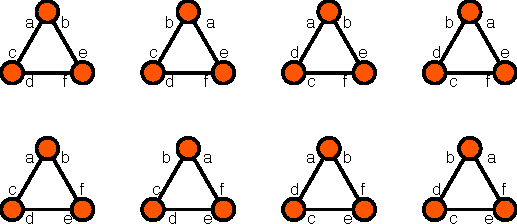
\includegraphics[height=2.4cm]{images/configuration_model_six_stubs.pdf}
\caption{}
\label{fig:reshuffle_simple_graphs}
\end{subfigure}
\begin{subfigure}[t]{0.45\textwidth}\centering
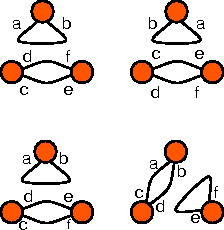
\includegraphics[height=2.4cm]{images/configuration_model_three_stubs.pdf}
\caption{}
\label{fig:reshuffle_loopy_multigraphs}
\end{subfigure}
\caption{Twelve of the ninety different possible rewirings of a triangle graph in the configuration model. In (a) only rewirings leading to simple graphs are considered. In (b) just four rewirings leading to loopy-multigraphs are shown.}
\label{fig:configuration_model_stubs}
\end{figure}
An approach that allows to get the right configuration model depending on the class of graph under exam, relies on the computational simulation of the correct rewiring probability by means of Markov Chain Monte Carlo algorithms, as proposed in~\cite{fosdick2016}.
In the remaining paragraphs, although flawed, we'll use the classic configuration model from Eq.~\ref{eq:configuration_model_probability} to be adherent to most of the brain networks literature, justified also by the vanishing effects of self-loops in large sparse networks. Nonetheless, we will illustrate many of the problems that the noncritical use of Modularity with this null model has introduced.

\subsection{Other null models for Modularity}
Modularity identifies communities as the subset of nodes whose internal fraction of edges deviates from the null configuration model on the same subset with the term $m_c/m > (K_c/2m)^2$.
Despite measuring deviation from a null model, Modularity does not take into account the statistical evidence associated with this deviation. For this reason, Modularity is not able to separate actual communities from those arising only from statistical fluctuations of the null model. Even worse, Modularity can find high-scoring partitions in fully random graphs~\cite{guimera2004} and in artificially built graphs with no community structure~\cite{kehagias2013}.

The configuration model is not the only possible null-model to use in spin-glass based quality functions. Different authors proposed several variants of Modularity~\cite{ronhovde2010,ronhovde2009,traag2011} with different null models.
The simplest variation of Modularity is the so-called ER Modularity~\cite{traag2015} that instead of the configuration model uses an Erd\H{o}s-Rényi random graph in which every edge appears with the same probability $p_{\textrm{ER}}$. The number of expected edges $\left< m_c \right>$ in a community of size $n_c$ is thus (in the space of simple graphs):
\begin{equation}
\left< m_c \right> = p_{\textrm{ER}}\binom{n_c}{2}.
\end{equation}
and plugging this null model into the RB model of Eq.~\ref{eq:rbspinglass2} we obtain the model:
\begin{equation}\label{eq:ermodularityrb}
\mathcal{H}^{ER} = -\sum \limits_c^C \left[\frac{m_c}{m}  - p_{\textrm{ER}}\binom{n_c}{2} \right].
\end{equation}
As the most similar ER graph of a given graph is the one that matches its density, the probability parameter $p_{\textrm{ER}}$ must be set equal to the original empirical graph density $\rho$. The so-called ER Modularity is derived by plugging the graph density in Eq.\ref{eq:ermodularityrb} and inverting its sign: 
\begin{equation}
Q^{ER} = \sum \limits_c^C \left[\frac{m_c}{m}  - \rho \binom{n_c}{2} \right].
\end{equation}
Under this model a group of nodes forms a community if its internal density is greater than the graph density $\rho$, on average.
Interestingly, from a machine learning perspective, all spin glass models quantify the discrepancy between observed and expected intramodular fraction of edges by means of a linear loss function. Among all the loss function, the linear is not the only possible and loss functions that take into account the relative size of clusters are possible.

\subsection{Beyond Modularity: Infomap}
Infomap is a method that has its bases\todo{descrivere brevemente infomap}

\section{Resolution limit}\label{sec:resolutionlimit}
Modularity attracted a lot of attention over the years as it became the tool of election to inspect the community structure of networks.
On one side, the wide use of Modularity, led many researchers to gain interest in complex networks, with results in sociology~\cite{li2008tag}, bioinformatics~\cite{saracc2012topology} and ICT~\cite{java2007we,leskovec2007dynamics}, just to mention a few, but on the other side, it offered a fallacious view on the community detection problem.
Indeed, although simple in many sense, Modularity optimization was hiding a problem that heavily limits its use in real world networks.

In 2007, a seminal article by Fortunato and Barthelemy~\cite{fortunato2007} did a thorough analysis of Modularity.
Their work showed the inability of Modularity to correctly identify communities that are smaller than a certain scale, determined by the square root of the number of edges. They dubbed this general phenomenon \emph{resolution limit}.
To illustrate what is meant by the resolution limit, here we follow the example of Fortunato and Barthelemy, with some obvious notational change.

Let us consider a toy network, $G=(V, E)$ that is composed of three subnetworks, as shown in~\ref{fig:figure_1_barthelemy}A.
The first subnetwork, a subgraph $G_0$ with $n_0$ nodes and $m_0$ edges is connected to two cliques, $G_1$ and $G_2$ by $m_{01}$ and $m_{02}$ links respectively. The two cliques are also connected by a number of $m_{12}$ links as shown in Figure~\ref{fig:figure_1_barthelemy}.
While $G_1$ and $G_2$, are complete subgraphs and are expected to be modules by construction, $G_0$ may consist of many communities. Maximum Modularity partitions then, should identify $G_1$ and $G_2$ as communities, independently from $G_0$.
To be more specific, let the partition where the two cliques are separated be denoted by $A$, with Modularity value $Q_A$. On the other hand, the partition where the two cliques are merged into a single community is denoted by $B$, with Modularity value $Q_B$.
To ease the calculations, we indicate the number of links $m_{12}$ as functions of $m_1$ and $m_2$, such that $m_{12}=a_{1}$, $m_1=a_2 m_2$, $m_{01}=b_1 m_1$ and $m_{02}=b_2 m_2$ with $a_1,a_2,b_1,b_2 \geq 0$.

As Modularity is a sum over the modules, and the module $G_0$ has the same Modularity $Q_0$ in both partitions, we are interested in studying the difference $\Delta Q = Q_{A} - Q_{B}$. After some simple algebraic manipulations it results:
\begin{equation} \label{eq:resolution_limit_delta}
\Delta Q = \frac{2 m a_1 m_1 - (a_1+b_1+2)(a_2+b_2+2)m_1 m_2}{2m^2}
\end{equation}
Specifically, we want to check when $\Delta Q > 0$, i.e. when the partition $A$ has a higher Modularity than partition $B$. This condition is verified as long as
\begin{equation}
m_2 < \frac{2m a_1}{(a_1+b_1+2)(a_2+b_2+2)}.
\end{equation}
In the case where $a_1=a_2=0$, there are no links between $G_1$ and $G_2$ and the condition is satisfied. When instead the two subgraphs are connected ($m_{12} \neq 0$), it happens that at some values of $m_1$ and $m_2$, the partition where the two modules are merged is preferred, i.e. $\Delta Q <0$. This means that when maximizing $Q^N$ on a network, is possible to miss some important structures, if they are too small.
More specifically, if the two modules have the same size and one sets $a_1=a_2=b_1=b_2=1/m$, is easy to check that Eq.~\ref{eq:resolution_limit_delta} is not satisfied if the number of links in the modules $m_c$, is lower than the square root of the total number of links in the network:
\begin{equation}
m_c < \sqrt{\frac{m}{2}}.
\end{equation}
To make this example more concrete we studied numerically a toy network where the three subgraphs take a precise form.
For the sake of illustration, we have defined $G_1$ and $G_2$ as two identical cliques of $5$ nodes connected to $G_0$ by a single edge ($m_{01}=m_{02}=1$) and to each other by $m_{12}$ edges.
The module $G_0$ was defined as a clique of variable size with a number of edges ranging from 45 to 2775. We then computed the numerical difference $\Delta Q$ and plotted it as a function of the number of edges $m_0$ in the $G_0$ clique.

\begin{figure}[htb!]
\centering
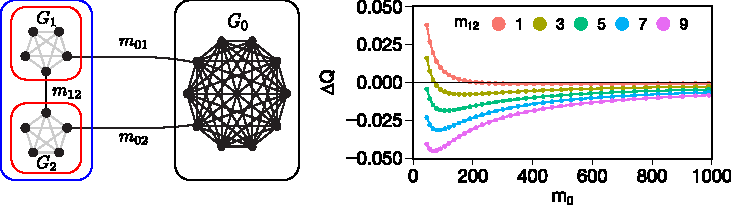
\includegraphics[width=1\textwidth]{images/barthelemy_modularity.pdf}
\caption{Analysis of the onset of the resolution limit for Modularity in a model graph (A) consisting of two cliques, $G_1$ and $G_2$, and a size-varying components $G_0$. The red line indicates the partition $A$, with $G_1$ and $G_2$ as different modules, and the blue line the partition $B$, with $G_1$ and $G_2$ merged into a single module. The graph (B) shows the difference in Modularity for increasing number of edges in $G_0$.}
\label{fig:figure_1_barthelemy}
\end{figure}

The onset of the resolution limit occurs when $\Delta Q$ changes sign and becomes negative for increasing values of $m_0$.
For $m_{12}=1$, i.e. when the two cliques $G_1$ ad $G_2$ were connected by only one edge (red curve), $Q$ showed this sign inversion for $m_0 \approx 200$ (Figure \ref{fig:figure_1_barthelemy}B).
With an increasing number of intercluster edges $m_{12}$, the resolution limit appeared for smaller and smaller values of $m_0$, eventually leading to $\Delta Q$ values that were always negative, i.e. the two cliques $G_1$ and $G_2$ were always merged by Modularity optimization.
An even more striking example of how the resolution limit affects Modularity is when looking at the optimal partition of a synthetic lattice graph, known as ``ring of cliques'', a network made out of identical cliques, connected in a ring-like structure by single links, as shown in Figure~\ref{fig:traag_ring_of_cliques}. 

\begin{figure}[htb!]
\centering
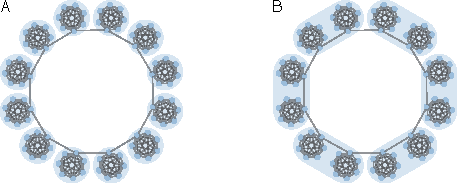
\includegraphics[width=1\textwidth]{images/traag_ring_of_cliques.pdf}
\caption{In this toy network, the intracommunity density is the highest possible, while the intercommunity density is the lowest to keep the network connected. The correct community structure is clearly the one on left (A), but Modularity values is higher for the partition on the right (B), where pairs of cliques coalesce into separated communities.}
\label{fig:traag_ring_of_cliques}
\end{figure}
If the number of cliques is large enough (they are more than $\sqrt{m}$), Modularity optimization leads to a partition where the cliques are combined into groups of two or more. This phenomenon can be observed already when considering a ring of 30 cliques made of 5 nodes, when the optimal Modularity partition combines cliques in pairs.
Yet extending the number of cliques, Modularity may merge cliques into groups of three, fours etc.

\subsection{Resolution parameter}\label{sec:resolution_parameter}
Different authors proposed solutions that try to circumvent the resolution limit: from the introduction of a tunable parameter that enables analysis of the network at an adjustable resolution level~\cite{reichardt2006,ronhovde2010,yeo2011} to an adequate edge re-weighting to decrease its adverse effects~\cite{berry2011}.

In this sense, the most common tuning to the Modularity quality function is the one that takes in consideration a \emph{resolution parameter}.
From the definition of $Q^N$ is evident that is possible to tune the size of the detected modules by multiplication of the configuration null model by a constant factor $\gamma_{N} \in [0,1]$, resulting in a modified modularity $Q^N(\gamma)$:
\begin{equation}
Q^N(\sigma,\gamma) = \sum_c^C \left[ \frac{m_c}{m} - \gamma_{N} \left( \frac{K_c}{2m}\right)^2 \right].
\end{equation}
However, exact specification of $\gamma_{N}$ requires prior knowledge of the expected size of the communities.
Moreover, it has been shown~\cite{lancichinetti2011} that an adjustable resolution parameter may reduce the tendency to merge small clusters, but only at the cost of unduly splitting large clusters. 
Indeed this is due to two opposite coexisting effects: the tendency to merge small subgraphs, which dominates when the resolution is low and the tendency to split large subgraphs, which dominates when the resolution is high.

In benchmark networks with heterogeneous distributions of cluster sizes, the simultaneous elimination of both biases is not possible and multi-resolution modularity is not capable of recovering the planted community structure even in graphs where the ground-truth structure is evident.
Therefore, adjustment of the resolution parameter is an attempt to balance these two biases, but multi-resolution methods fail to recover community structures comprising heterogeneous distributions of cluster sizes~\cite{lancichinetti2011}. 

In another attempt to better tolerate the resolution limit, scholars applied appropriate techniques of edge re-weighting~\cite{berry2011} to enhance communities prior to Modularity maximization.
Although this technique proved able to better tolerate the detrimental effect of the resolution limit, it only shifted the scale of the problem.
After all, real-world networks are characterized by the coexistence of clusters of very different sizes, therefore no single parameter can adapt to the variety of network topologies observed in nature.

\subsection{Resolution-limit free quality functions}\label{sec:resolution_limit_free_quality_functions}
In an attempt to quantitatively characterize the resolution limit, Traag et al.~\cite{traag2011} proposed a rigorous definition of \emph{resolution-limit-free} graph partitioning.

A quality function is resolution-limit-free if, given an optimal partition $\zeta$ of a graph $G$, any module $\zeta_i$ is also optimal for the graph induced by the nodes in $\zeta_i$.
In other words, each community of the optimal partition is not split by optimization of the quality function applied to the subgraph induced by the nodes in the community.
Hence, each community does not depend on the rest of the network and is both locally and globally optimal.
Then, in order to design such resolution-limit-free quality function, Traag took a spin glass model, with a null model specified by constant quantity $\gamma_{\textrm{CPM}}$~\cite{traag2011} and dubbed it \emph{Constant Potts Model}.

The \emph{Constant Potts Model} (CPM) identifies community as subset of nodes whose internal density $\rho_c$ is bigger than the overall graph density multiplied by a factor $\gamma_{\textrm{CPM}}$ that defines the typical scale of the communities. In the framework of Reichardt and Bornholdt, the CPM model has the following Hamiltonian: 
\begin{equation}\label{eq:cpm_hamiltonian}
H(\sigma)^{\textrm{CPM}} = - \sum \limits_{(i,j) \in V^2} \left[ a_{ij} - \rho \gamma_{\textrm{CPM}} \right] \delta(\sigma_i,\sigma_j),
\end{equation}
that once reworked in an additive quality function, results in the form of Eq.~\ref{eq:cpm_hamiltonian} 
\begin{equation}\label{eq:cpm_ermodel}
Q^{\textrm{CPM}} = \sum \limits_c^{|C|} \left[m_c - \gamma_{\textrm{CPM}} n_c^2 \right] 
\end{equation}
In other words, the model tries to maximize the number of internal edges while at the same time keeping relatively small communities. The parameter $\gamma_{\textrm{CPM}}$ balances these two imperatives acting as the inner and outer threshold of edge density.
Hence, in the CPM settings is better to split two communities $r$ and $s$ if $\gamma_{CPM}$ exceeds the inter-community density $m_{r,s}/(2n_r n_s)$.

Unfortunately, the operation of tuning the resolution parameter, both in the CPM model as well as in other similar models, is difficult and no largely accepted method exists, making all the models based on a resolution parameter, scarcely used in practical applications.


\subsection{Effects of resolution limit}
In the context of brain networks, the resolution limit first highlighted by Fortunato and Barthelemy may be particularly critical for the analysis of brain connectivity networks, as it may unduly merge modules that are too small, therefore hampering the ability to highlight regions of functional segregation from the rest. Indeed, there are some functional processes in the brain that are thought to be better represented as anatomically localized like the first stages of sensory processing, while others are seen as more globally integrated processing system, in particular attentional processes~\cite{alnaes2015}.
Hence, we may expect the brain modular structure to comprise communities of heterogeneous dimensions.
Whether the relatively uniform modular structure of brain connectivity, highlighted by Newman's Modularity and other community detection methods in many studies, reflects the true architecture of the brain organization or is the result of the resolution limit is still unclear~\cite{nicolini2016}.
Hierarchical approaches have shown that large modules can be further subdivided, indicating that connectivity networks show structure at different spatial scales~\cite{meunier2009}.
However, these findings do not provide information on the optimal partition of the network, i.e. the optimal cut through the dendrogram representing connectivity at the different scales.

Thus, the resolution limit is a critical shortcoming for the study of brain networks and likely influenced many studies in the literature.
The limitation on the number of detected modules in brain networks is evident in studies where typically four or five communities of the same size are detected in humans, as in Crossley et al.~\cite{crossley2013a}, Meunier et al.~\cite{meunier2009a,meunier2010}, Fair et al.~\cite{fair2009} or also in mouse models~\cite{schwarz2008}.
To this end, an optimization method that does not suffer from the resolution limit would be needed.

It's also very important to stress that comparing the Modularity value $Q^N$ across different networks obtained in different studies, with possibly a different number of nodes or different densities is an erroneous practice although $Q^N$ is normalized in the range $[0,1]$. As shown by a number of studies~\cite{good2009,kehagias2013,radicchi2010}, even in graphs which do have a natural community structure, high modularity values can be achieved by partitions which do not respect this natural structure. Hence, the Modularity value is only a numerical indication of the current status of optimization of the detected community structure on a specific graph and should never be confronted across different networks.


%%%%%%%%%%%%%%%%%%%%%%%%%%%%%%%%%%%%%%%%%%%%%
%%%%%%%%%%%%%% DEGENERACY %%%%%%%%%%%%%%%%%%%
%%%%%%%%%%%%%%%%%%%%%%%%%%%%%%%%%%%%%%%%%%%%%
\section{Degeneracy}\label{sec:degeneracy}
The differences in Modularity between optimal and suboptimal partitions can be very small, as observed in Figure~\ref{fig:figure_1_barthelemy}B, where $\Delta Q$ between the two partitions with split or merged cliques, remains close to zero for a large range of $m_0$ especially at $m_{12}=1$.
Indeed, even in the case where it would not be beneficial for Modularity to merge two modules, i.e $\Delta Q <0$, this difference can be made arbitrarily close to zero.

The total number of different partitions in a graph is the Bell number $B_n$~\cite{stanley1997} and it grows faster than exponentially in $n$, therefore a combinatorially large number of sub-optimal partitions exist around the global optimum. These partitions may be very close in terms of Modularity to the optimum but radically different in terms of similarity.
Thus, counter-intuitively, when the network becomes more modular, the globally optimal partitions becomes harder to find among the growing number of suboptimal but competitive alternatives.

This consideration explains the empirical observation that nearly-optimal solution tend to group into high-modularity plateaus, although they may differ substantially~\cite{good2009}. This phenomenon, dubbed \emph{degeneracy} affects Newman's Modularity and probably many other spin-glass based quality functions.
As a matter of example, the variation in Modularity for merging a pair of adjacent cliques in the ring of cliques graph shown in Figure~\ref{fig:traag_ring_of_cliques}, is given by:
\begin{equation}\label{eq:modularity_difference_ring_clique}
\Delta Q = \frac{1}{r\left(\binom{n_r}{2}+1\right)}-2r^{-2}
\end{equation}
where $r$ is the number of cliques and $n_r$ the number of nodes in each clique.
In the large $r$ limit, the difference in Eq.~\ref{eq:modularity_difference_ring_clique} tends to a small negative value, indicating that a solution where the cliques are merged, may have a Modularity very close to the optimum. Indeed, already for $r=20$ cliques, $\Delta Q \approx 5\times 10^{-3}$, making all the suboptimal partitions where cliques are merged, very close to the optimal solution.

To make this argument more intuitive, we extrapolated a visually appealing form of the complex landscape of partitions' Modularity for a ring of cliques network. We sampled the configuration space of the partitions of a ring of clique network through a Montecarlo procedure and annotated the corresponding values of Modularity for every partition as in~\cite{good2009}.
We then built a similarity matrix between all sampled partitions and embedded it into a three-dimensional space maintaining similarity relations between partition following a Curvilinear Components Analysis (CCA).
In the embedded manifold, two partitions are close if they are similar and the z-axis encodes the quality function.
A highly degenerate plateau can be observed in~\ref{fig:degeneracylandscape} whereby different solutions with high values of Modularity stay in the same neighborhood.

\begin{figure}[htb!]
\centering
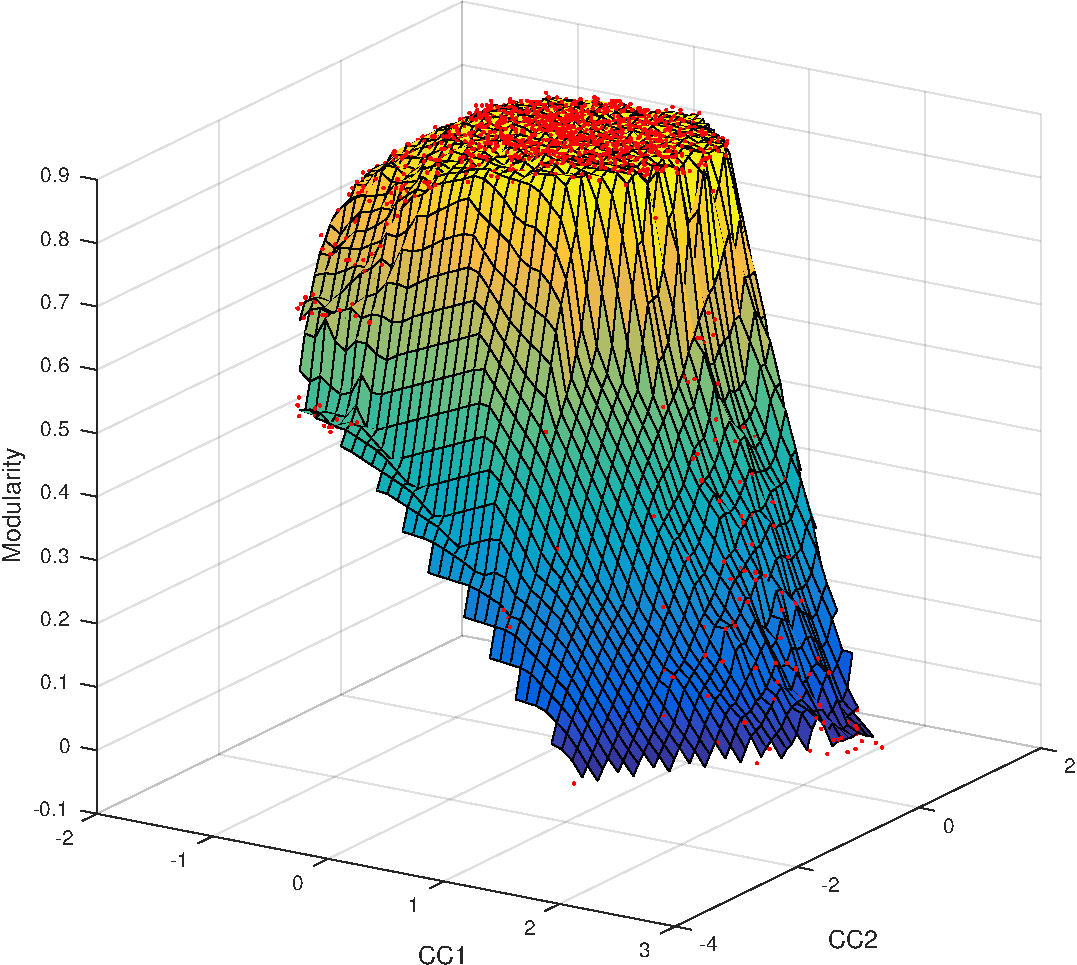
\includegraphics[width=0.75\textwidth]{images/degeneracy_modularity.pdf}
\caption{Degeneracy landscape for Newman's Modularity in a ring of cliques with $r=24$ cliques of $n_r=5$ nodes. The axes CC1 and CC2 are complicated functions of the original partition space computed as to maintain the distance relation between points and their scale is unimportant.}
\label{fig:degeneracylandscape}
\end{figure}

Any quality function suffering degeneracy of solutions should display an embedded landscape with a plateau of optimal partitions, like the one shown in Figure~\ref{fig:degeneracylandscape}, while in the case of the existence of a distinct global optimum, a sharper peak should be exhibited.
We'll see that recasting the problem of community detection in terms of probability theory, will help in the definition of a quality function showing convex behaviour and uniqueness of the optimum solution.

The issue of degeneracy is not only affecting Newman's Modularity $Q^N$ but other quality functions as well.
In this respect, it's clear that choosing the partition with the highest quality value isn't meaningful and a choice that considers all the good partitions at the plateau is desired. 
An optimal partition of the network can then be expressed as a \emph{median} of the solutions over the optimal plateau.
This approach, known as \emph{consensus clustering}, is advantageous to combine strengths and weakness of found partitions, whereby some local effects of noise during optimization are averaged over a large set of solutions.
Such approach for consensus clustering is typically based on a meta-algorithm rather than a proper community detection method. Indeed, given a community detection method, consensus clustering forms an ensemble of optimal solutions from which an association matrix $\mathcal{A}$ is computed, where edges are proportional to the probability that two nodes are connected in the same community. 
Consensus communities are then obtained clustering iteratively the thresholded association matrix. The choice of the threshold that makes the association matrix sparser~\cite{lancichinetti2012} is dictated by the properties of the chosen method of community detection itself. Typically with a smartly chosen threshold, consensus clustering converges in a few iterations. The pseudo-code illustrated in Alg.~\ref{alg:consensus_clustering} illustrates all the steps of consensus clustering.

\begin{Algorithm}[htb!]
\begin{codebox}
\Procname{\proc{ConsensusClustering}(a graph $G$, a community detection method)}
\li Apply community detection on $G$ for $n_p$ times, yielding $n_p$ partitions.
\li Compute the consensus (association) matrix $\mathcal{A}$ where $\mathcal{A}_{ij}$ is the probability \\that vertex $i$ and $j$ are assigned in the same community over $n_p$ partitions.
\li Threshold the association matrix $\mathcal{A}$ with a parameter $\tau$.
\li Apply community detection on $\mathcal{A}$ for $n_p$ times to yield $n_p$ partitions.
\li If $\mathcal{A}$ is block diagonal (all partitions are equal) stop, else return to 1.
\end{codebox}
\caption{Pseudocode for the implementation of consensus clustering.}
\label{alg:consensus_clustering}
\end{Algorithm}

Although useful to address the degeneracy issue, this approach keeps suffering the resolution limit, as the sub-optimal optimal solutions which the consensus partition is made of, are themselves resolution-limited.

% \section{Alternative approaches to Modularity}
% If the problems of Modularity are evident, researchers tried to mitigate them with alternative meta-approaches. The issue of degeneracy indeed, implicitly maintains that in the absence of a clearly optimal partition, many partitions should be used instead. Yet, the problem of the resolution limit that arises from an inadequate choice of the configuration model as the null hypothesis, can be tackled by a proper choice of the null model that keeps into account the sources of random noise directly from the time series which the correlation matrix is originated from. Here we briefly discuss these two potential solutions to the problems we have just introduced.

% \subsection{Consensus clustering}

% \subsection{The bias of the null model for Modularity}
% The null model of Modularity is not only is at the basis of the issues of resolution limit and degeneracy, but can be shown to be highly inadequate when used in brain networks based on estimates of Pearson correlation of BOLD time series.
% As shown by MacMahon and Garlaschelli~\cite{macmahon2015}, indeed the configuration model introduces a systematic bias as it is not consistent with the definition of Pearson correlation.
% Ideally, the modular structure in a full correlation matrix (a correlation matrix with all nonzero entries) should reflect a balance between positively and negatively correlated units. Correlation communities should be internally positively correlated while externally negatively correlated, but this does not happen when naively applying Modularity to correlation-based networks.
% Such inadequacy results from a systematic bias that the configuration model introduces, here shortly explained.

% Given $n$ time series $\mathbf{X}=\{ X_1, \ldots, X_n\}$ from the parcellation atlas, the Pearson correlation matrix is computed as
% \begin{equation}
% C_{ij} = \frac{\textrm{Cov}(X_i,X_j)}{\sqrt{\textrm{Var}(X_i)\textrm{Var}(X_j) }}.
% \end{equation}
% A naive application of Newman's Modularity to such correlation matrix results in:
% \begin{equation}
% Q^N= \frac{1}{C_{\textrm{norm}}} \sum \limits_{ij} \left[ C_{ij} - \langle C_{ij} \rangle \right] \delta(\sigma_i,\sigma_j) = \left[ C_{ij} - \frac{k_i k_j}{C_{\textrm{norm}}} \right] \delta(\sigma_i,\sigma_j)
% \end{equation}
% where $k_i=\sum_{j=1}^n C_{ij}$. Unfortunately though, this last term is biased because expanding the terms $k_i$ one obtains:
% \begin{equation}
% k_i =\sum_{j=1}^n C_{ij}= \sum_{j=1}^n \textrm{Cov}(X_i,X_j) = \sum_{j=1}^n \textrm{Cov}(X_i,X_{tot})
% \end{equation}
% where $X_{tot}=\sum_{j=1}^n x_j$ has zero mean but non unit variance, and the configuration model naively applied to correlation matrices becomes:
% \begin{equation}
% \frac{k_i k_j}{2m} = \textrm{Corr}(X_i,X_{tot})\textrm{Corr}(X_j,X_{tot})
% \end{equation}
% Such badly-adapted configuration model does not give more importance to pairs of strongly correlated time series but rather to pairs of time series whose direct correlation $C_{ij}$ is larger than the common signal $X_{tot}$.
% The null model proposed by MacMahon and Garlaschelli redefines the null model of Modularity to take into consideration such desired property. Thanks to the \emph{random matrix theory} the bulk of signal due to the global mode, a large-scale oscillation that positively correlates all areas, is removed and only terms that retain true correlations are maintained.

\section{Quality function optimization}
\subsection{Louvain method}\label{sec:louvain_method}
Optimization of fitness function in the additive form of Eq.~\ref{eq:rbspinglass2} is typically performed using the Louvain method~\cite{blondel2008}, a greedy agglomerative clustering algorithm that works on hierarchical refinements of the network's partitions. The inspiration for this method of community detection is the optimization of Modularity as the algorithm progresses. In the Louvain method of community detection, first small communities are found by optimizing modularity locally on all nodes, then each small community is grouped into one node and the first step is repeated.
\todo{aggiungere louvain non deterministico}
This algorithm has become extremely popular in recent years because it is fast, allowing to analyze huge networks with billions of edges and produces significant partitions~\cite{lancichinetti2009}.  The optimization method is divided in two phases applied recursively as depicted in Figure~\ref{fig:louvain_method}. The first phase is the optimization phase which looks for a locally optimal partition by considering only individual vertex swaps. As in many other greedy algorithms, the community partition is initialized with a single node per community and as many communities as nodes in the input network. Then, based on the chosen cost function, individual nodes are removed from their current community and swapped to the neighboring community which produces the largest positive gain of the cost function.

\begin{figure}[htb!]
\centering
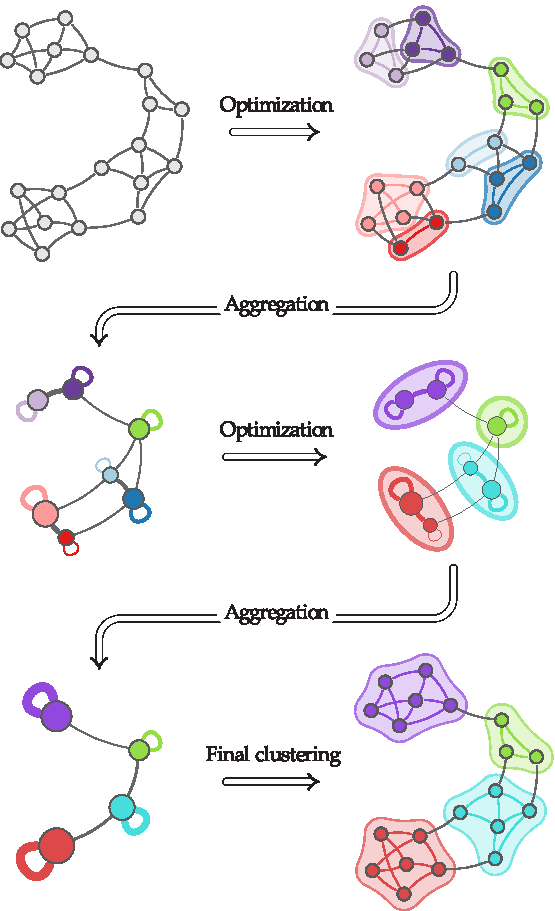
\includegraphics[width=0.6\textwidth]{images/louvain_method.pdf}
\caption{Optimization and aggregation steps with the Louvain method. Figure taken from~\cite{browet2014}.}
\label{fig:louvain_method}
\end{figure}

\subsection{Spectral optimization}
Another (and earlier) method to optimize Modularity is the spectral Modularity by Newman. Given the form of Modularity as in Eq.~\ref{eq:newmanmodularityspinglass}, one calls the modularity matrix the quantity $\mathbf{B}=A_{ij} - k_i k_j/2m$. From it, it's possible to obtain an equivalent linear algebra formulation of Modularity that reads:
\begin{equation}\label{eq:newman_spectral}
Q^N = \frac{1}{4m} \mathbf{s}^T \mathbf{B} \mathbf{s}
\end{equation}
where $\mathbf{s}$ is a numerical vector that considers a division of the network in two communities, with values $s_i=+1$ if vertex $i$ belongs to group 1 and $s_i=-1$ if vertex $i$ belongs to group 2. With some manipulations~\cite{newman2006,newman2010book}, the Modularity maximization is turned into an symmetric eigenvalue problem of the form
\begin{equation}
\mathbf{B} \mathbf{s} = \beta \mathbf{s}.
\end{equation}
The group assignment of each node is obtained as the signs of the eigenvector $\mathbf{s}$ corresponding to the greatest eigenvalue $\beta$. Finally, by repeatedly subdividing the network, the optimal Modularity assignment is recovered~\cite{newman2006,newman2010book}.

